\documentclass[12pt]{article}

\usepackage{graphicx}
\usepackage{tikz}
\usepackage{array}

\title{AMath Tea Time --- Puzzle \#8}
\author{}
\date{\vspace{-1cm}2 June 2015}

\begin{document}

\maketitle
\pagenumbering{gobble}

\subsection*{Problem}

A casino machine accepts tokens of 32 different colors, one at a time. For each
color, the player can choose between two fixed rewards. Each reward is up to
\$10 cash, plus maybe another token. For example, a blue token always gives the
player a choice of getting either \$5 plus a red token or \$3 plus a yellow
token; a black token can always be exchanged either for \$10 (but no token) or
for a brown token (but no cash). A player may keep playing as long as they have
a token. Rob and Bob each have one white token. Rob watches Bob play and win
\$500. Prove that Rob can win at least \$1000.

\begin{figure}[ht]
  \centering
  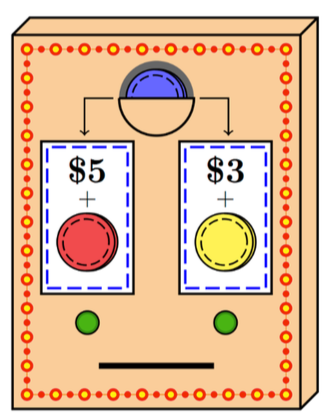
\includegraphics[height=140px]{casino.png}
\end{figure}

\subsection*{Hints}

{
\par\vspace*{\fill}
\noindent \small \it
If you have any puzzles to share then send them my way at {\tt
  cswiercz@uw.edu}!
}

\end{document}
